\chapter{Asking Billionaires How They Got Rich (Houston)}

This lecture is mathematically serious in a different way from a blackboard lecture. We are not deriving a field equation; we are extracting the arithmetic that lies underneath entrepreneurial scale. The host begins with spectacle---names, billion-dollar claims, startling profit figures---and then resets the problem. What, step by step, turns a tiny initial position into durable scale? As the lecture unfolds, the answer comes in layers: capital, margin, reinvestment, profitability, systems, timing, standards, and the discipline not to confuse appearance with strength.

\section{Headline Claims and the Question They Create}

The lecture opens with a cold prologue of later headline claims. The point is not yet explanation; it is to establish scale large enough to demand explanation. Among the prologue quantities are

\begin{align}
N_{\text{female founders}} &= 20,\\
\sum_{i=1}^{76} V_i &= \$1.27\ \text{billion},\\
\Pi_{\max} &= \$980\ \text{million}.
\end{align}

These numbers arrive before their mechanisms. Only then does the host reset at the Aspire Tour in Houston and state the governing question: we are here to learn how wealth was created and what advice remains usable for people trying to build large businesses now.

We should keep that order. First the lecture shows us magnitude; then it asks what produced it. The entire chapter grows out of that turn from spectacle to mechanism.

\section{Kendra Scott: Bootstrap Growth, Margin, and Delayed Capital}

The first full case is Kendra Scott. The host asks the familiar sequence of questions---who are you, what industry did you choose, are you a business owner---and quickly narrows to the central claim: she is one of only twenty female founders in the United States to have built a billion-dollar brand. The next question is the right one: what is the secret?

Scott does not begin with institutional capital or a polished business plan. She begins with a first collection made from \(\$500\). To translate her story into a clean bookkeeping model, let \(C_t\) be working capital in cycle \(t\), \(R_t\) sales, \(m_t\) the usable gross margin rate, \(O_t\) operating costs, \(B_t\) borrowed capital, and \(B_t^{\text{serv}}\) the cost of servicing that borrowing. Then the lecture's growth mechanism may be written as

\begin{align}
C_0 &= \$500,\\
K_t^{\text{ext}} &\approx 0 \qquad \text{for roughly the first decade},\\
E_t &= m_t R_t - O_t - B_t^{\text{serv}},\\
C_{t+1} &= C_t + E_t.
\end{align}

This is a cautious reconstruction, not a visible board equation. But it is faithful to the spoken sequence: make the first collection, write orders, keep enough margin, reinvest, and use debt when no outside investor will provide equity.

A useful consequence follows immediately by iteration:
\begin{equation}
C_n = C_0 + \sum_{t=0}^{n-1} E_t.
\end{equation}
That is the entire bootstrap story in one line. In a founder-financed regime, future capacity is the initial capital plus accumulated reinvestable earnings. The lecture does not give us exact values of \(m_t\), \(O_t\), or \(B_t^{\text{serv}}\), so we do not pretend to know them. What matters is the sign and persistence of \(E_t\).

\begin{proposition}
If outside capital remains absent for an extended period, then durable expansion requires positive reinvestable earnings over enough business cycles.
\end{proposition}

\begin{proof}
From
\[
C_n = C_0 + \sum_{t=0}^{n-1} E_t,
\]
we see that working capital cannot expand unless the cumulative sum of reinvestable earnings expands. If \(\sum_{t=0}^{n-1} E_t\) remains too small, or becomes negative after debt service and operating costs, the business cannot finance a larger next cycle from its own activity. In that case it must shrink, borrow more aggressively, or stop. Thus in a long bootstrap period, positive reinvestable earnings are not decorative; they are the condition of continued scale.
\end{proof}

Scott then adds the harsher details that make the recurrence real. For ten years no investor gave her money. She used a line of credit, credit-card debt, and collateralized everything she owned. The update rule therefore lives under pressure:
\begin{equation}
C_{t+1}=C_t+\bigl(m_tR_t-O_t-B_t^{\text{serv}}\bigr),
\end{equation}
and the founder survives only if the business can keep producing enough substance to feed the next cycle.

\begin{figure}[h]
\centering
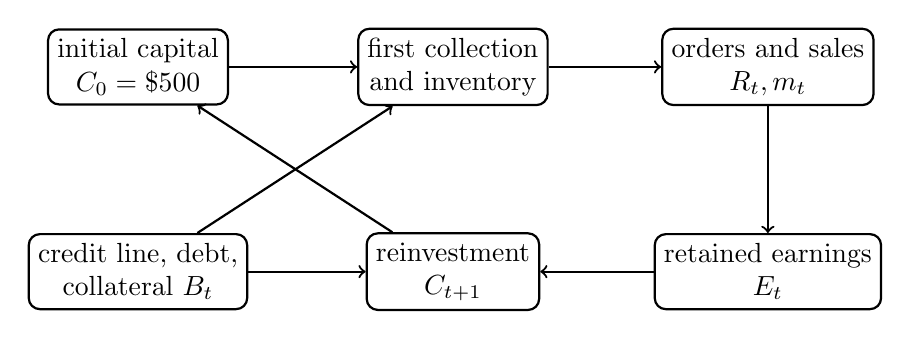
\begin{tikzpicture}[thick]
\node[draw, rounded corners, align=center] (c0) at (0,0) {initial capital\\\(C_0=\$500\)};
\node[draw, rounded corners, align=center] (prod) at (4,0) {first collection\\and inventory};
\node[draw, rounded corners, align=center] (sales) at (8,0) {orders and sales\\\(R_t,m_t\)};
\node[draw, rounded corners, align=center] (earn) at (8,-2.6) {retained earnings\\\(E_t\)};
\node[draw, rounded corners, align=center] (reinv) at (4,-2.6) {reinvestment\\\(C_{t+1}\)};
\node[draw, rounded corners, align=center] (debt) at (0,-2.6) {credit line, debt,\\collateral \(B_t\)};

\draw[->] (c0) -- (prod);
\draw[->] (prod) -- (sales);
\draw[->] (sales) -- (earn);
\draw[->] (earn) -- (reinv);
\draw[->] (reinv) -- (c0);
\draw[->] (debt) -- (prod);
\draw[->] (debt) -- (reinv);
\end{tikzpicture}
\caption{Editorial schematic of the bootstrap loop described in the Kendra Scott segment. No board figure survives; this diagram simply organizes the spoken mechanism.}
\end{figure}

Only after visible traction appears---lines around the block, people coming in, unmistakable demand---do private-equity and venture-capital firms begin calling. In the arithmetic of the lecture, outside capital is not the cause of traction. It is attracted by traction.

\subsection{Question \& Answer}

\paragraph{Question.} Why does profitable traction matter more than an impressive top line when outside capital is absent?

\paragraph{Answer.} Because in that regime the business has to propagate itself through genuine operating surplus rather than through reputation. Scott says this directly: build a profitable business, not merely one that looks good on the top line. In compact form,
\begin{equation}
\text{top line} \not\equiv \text{healthy business},
\qquad
\mathrm{EBITDA}>0.
\end{equation}
The inequality is editorial shorthand, but it captures the lecture's force. Revenue may advertise the business; earnings finance the next cycle. The investors come later, when the business has already demonstrated that it can turn activity into durable surplus.

\section{Confidence, Anti-Intimidation, and Negotiation as Research}

The lecture now changes gears. Having explained a finance mechanism, it asks what kind of person can carry that mechanism through rooms full of power. Scott is asked about the best advice she received from a mentor, and she rejects the familiar slogan that we must simply fake it until we make it. The operative rule is subtler: do not be intimidated.

Here the lecture is careful. Confidence is not offered as theater. It is the behavioral form taken by preparation. Scott says she has entered many rooms in which no one looked like her, and the answer was not performance for its own sake but a settled knowledge that she knew what she was talking about and would not allow herself to be shrunk.

The negotiation segment sharpens the point. She says she comes in as a sponge; she wants to hear the other side. But she also comes in prepared. She knows who will be sitting in the room, what their backgrounds are, what other deals they have done, and what others have learned from negotiating with them. Thus negotiation in this lecture is not bluster. It is informed asymmetry. One listens, studies, and then surprises the counterparty at the moment when surprise matters.

At the end of the segment, the host performs a brief recap, converting the interview into portable advice for the audience. That recap is part of the lecture's rhythm. The voice moves from one person's story to a general principle: go into the room prepared to win, regardless of who sits across from you.

\section{From One Company to Many: Systems, Process, and Diversification}

After the Kendra Scott recap, the lecture widens. The host stops a private-equity operator and moves from the arithmetic of one brand to the arithmetic of many businesses under one operating logic. The interview quickly lays out the portfolio claim: in 2019, \(76\) companies were sold for \(\$1.27\) billion, and the same speaker later says he runs \(86\) companies at the same time.

The essential mathematical move here is not the large number itself but the mechanism of replication. The speaker says diversification becomes rational only when a process is replicable. Let \(P\) be a common operating process, \(D\) a centralized data layer, \(M_i\) empowered managers, and \(L_i\) the business units. Then the lecture's architecture can be summarized by
\begin{align}
N_{\text{portfolio}} &= 86,\\
(P,D,\{M_i\}_{i=1}^N) &\Rightarrow \{L_i\}_{i=1}^N.
\end{align}

The point is not that one heroic individual personally performs \(N\) businesses. The point is that the founder sits at the architecture layer. Data rises upward, decisions are distributed, and the same system is reused across different operating contexts.

This interview also adds two motivational qualifiers that matter. First, not everyone is built for entrepreneurship. The lecture refuses the flattening belief that desire alone is enough; it insists on grind and process. Second, the operator recommends AI and tech because they presently offer the greatest opportunity for scale. We need not formalize that recommendation into a theorem. It is enough to observe that, in the lecture's logic, scale is tied to repeatability and leverage.

\subsection{Question \& Answer}

\paragraph{Question.} When does diversification become a rational extension of a system rather than a distraction from the core business?

\paragraph{Answer.} Only when the core business has become legible as a repeatable operating structure. The lecture says this plainly: when you have a system and process that is replicable, the same logic can be used again and again. In shorthand,
\begin{equation}
\text{replicable process} \Rightarrow \text{diversifiable operating model}.
\end{equation}
Without that portability, diversification multiplies confusion. With it, diversification is simply repetition at a larger scale.

\section{Family Capital, Audience Address, and the Trust Interlude}

At this point the lecture steps away from interviews. The host turns directly to the audience and talks about money not only as business fuel but as family stewardship. This is a sponsor interlude, but structurally it does real work. It broadens the lecture from enterprise capital to household capital.

The message is that making money work for us is one level of discipline, and making it work for our family's future is another. The lecture speaks of children's futures, long-term planning, and then, in a somewhat garbled but still intelligible passage, the need to be careful about the people one trusts: grants, people, employees, partnerships, and counterparties of all kinds.

We should not over-mathematize this section, because the transcript itself does not. But we should retain it. It changes the frame. Wealth is no longer only about scaling a business; it is also about allocating attention, trust, and capital across a household horizon.

\section{Marcus Lemonis and the Discipline of Substance}

The Marcus Lemonis segment consolidates many earlier threads. He begins with industry choice and says, in effect, that he wanted white space: a sector with few competitors and a clear consolidation opportunity. He then describes the scale of the result. Twenty years earlier, the business was effectively at zero. Later it became a \(\$7\) billion business:
\begin{align}
V_{\text{business}}(0) &\approx 0,\\
V_{\text{business}}(20\ \text{yr}) &= \$7\ \text{billion}.
\end{align}
This is the speaker's scale claim, not a formally verified value, but it serves the lecture's purpose: industry selection, when combined with consolidation and execution, can create enormous room for scale.

The interview then returns to profit and cyclicality. The most the company ever made in a single year, he says, was \(\$980\) million in profit. Yet he immediately adds the corrective: that does not always happen. There are good times and bad times, and the key is to find the middle and become comfortable there. This is an important rhythm in the lecture. A large number is stated, and then a stabilizing sentence arrives so that we do not worship the outlier and forget the cycle.

Next comes the team principle. Delegation matters, but more important is surrounding oneself with people who are smarter, willing to say no, and willing to challenge the founder when the founder is wrong. The lecture continues to move away from solitary heroics and toward a decision architecture in which better information can rise upward.

Finally, Marcus gives the lecture its sharpest risk principle. What keeps people broke, he says, is the urge to be flashier than they should be, to care more about what they look like than about what they are. If we write total capital deployment as
\begin{equation}
A = A_{\text{sub}} + A_{\text{flash}},
\end{equation}
where \(A_{\text{sub}}\) denotes productive allocation and \(A_{\text{flash}}\) status allocation, then the lecture's claim may be compressed as
\begin{equation}
A_{\text{flash}} \uparrow
\qquad \Longrightarrow \qquad
\text{financial fragility} \uparrow.
\end{equation}

This is not a theorem in the strict sense. It is an operational warning. Productive capital improves future earning power. Status capital raises expectations, fixed burn, and the pain of reversal. That is why Buffett is invoked. The old car and the old house are not moral props; they are signs of a life not structured around permanent symbolic overhead.

\subsection{Question \& Answer}

\paragraph{Question.} How do we enjoy success without making ourselves financially fragile?

\paragraph{Answer.} By preserving the distinction between comfort and theater. The lecture does not forbid having nice things. It forbids allowing symbolic expenditure to become the logic of the life. Once that happens, a setback threatens not only income but identity. Marcus's answer is to remain in the middle: substantial enough to be secure, restrained enough to remain resilient.

The host again pauses to recap. He tells the audience that the secret to building the larger company was not merely delegation but finding people smarter than oneself and letting them make the right decisions. This recap is worth keeping because it translates the interview back into the lecture's general language of scale.

\section{Timing, Health, Standards, and the Price of Value}

The closing movement is compact and pointed. Daymond John begins with two maxims. The first is that money is a great slave but a terrible master. The second is that pioneers get slaughtered while settlers prosper. The two belong together. Wealth is not merely a question of acquiring money; it is a question of not being mastered by it, and of understanding timing.

The timing principle can be written in very condensed form:
\begin{equation}
\text{too early} \Rightarrow \text{market does not yet understand the offer}.
\end{equation}
This is the lecture's way of saying that originality and timing cannot be separated. A pioneer may be right in substance and still lose because the market cannot yet read the offer. The settler arrives later, with a more legible version, and prospers.

Daymond then gives a striking answer to the question of becoming a multimillionaire. He changes the definition. If health is absent, the monetary label no longer captures the real condition. The lecture thereby places a bound on financial aspiration: a life unable to use its money is not the life being sought.

The final interview, with Billy Ray Taylor, narrows the lecture into standards. He offers the bird-and-branch analogy: the bird survives not because the branch is perfectly reliable, but because the bird trusts its wings. From there the lecture moves to deliberate clarity: you cannot manage a secret. A business owner for five years, Billy Ray says he branched off and started LinkedXL, and his personal annual income has fallen in the seven-figure range,
\begin{equation}
Y_{\text{Billy Ray}} \in [\$1\text{M},\,\$3\text{M}].
\end{equation}

The lecture then turns to a sharper lesson from his mother: start with a stand. The home plate in baseball is \(17\) inches wide, and the standard does not widen because a player wants relief. In the same spirit, price and worth do not become clearer when we blur them to avoid discomfort.

\subsection{Question \& Answer}

\paragraph{Question.} What is the difference between charging a price and stating a value proposition?

\paragraph{Answer.} The lecture answers with a worked sales arithmetic. Billy Ray says that when he gave away consulting and software for free, the market largely ignored him. When he priced the work and linked that price to the customer's possible gain, the same offer became legible as an investment. In the transcript's own numbers,
\begin{align}
\text{fee} &= \$5{,}000,\\
\text{claimed client gain} &= \$5{,}000{,}000,\\
\frac{\text{claimed client gain}}{\text{fee}} &= 1000.
\end{align}

The ratio is rhetorical, not audited. But it is exactly the kind of rhetorical arithmetic the lecture wants us to notice. A naked price sounds like cost. A value proposition frames the same price against the scale of the client's loss or upside. That is why Billy Ray keeps returning to worth, value, and standards: pricing is not only a number; it is a statement of what the work is for.

We may also hear the closing phrase \emph{deliberate clarity} as a summary of the whole lecture. Capital, process, health, timing, teams, and value all become more manageable once they are named plainly and measured against standards rather than fantasy.

\section{Summary}

The lecture begins with a trailer of giant outcomes and then slowly makes them intelligible. Kendra Scott gives us the bootstrap recursion: initial capital, margin, debt, reinvestment, and delayed investor arrival. The private-equity operator enlarges the frame from one business to many by insisting on process, data, and portability. The interlude on family capital reminds us that wealth is also stewardship. Marcus Lemonis turns scale into a lesson about resilience, substance, and the danger of living above one's durable baseline. Daymond John adds timing and health, while Billy Ray Taylor closes with standards, clarity, and value-based pricing.

What emerges is not one master formula but a family of operating rules. Capital must recycle. Profit must be real. Systems must be portable. Teams must be stronger than the founder's ego. Visible success must not outrun resilience. And price must be attached to value. In that sense, the lecture does not treat wealth as a mysterious event. It treats wealth as an ordered sequence of disciplined conversions:
\[
\text{capital} \to \text{margin} \to \text{reinvestment} \to \text{scale} \to \text{stewardship}.
\]
That is the arithmetic spine of the chapter.